\documentclass[12pt]{article}
\usepackage[utf8]{inputenc}
\usepackage{lipsum}
\usepackage{pifont}
\usepackage{outlines}
\usepackage{multirow}
\usepackage{subcaption}
\usepackage{adjustbox}
\usepackage{amsmath}
\usepackage{makecell}
\usepackage{fancyhdr}
\usepackage{float}
\usepackage{graphicx}
\usepackage{tikz,xcolor}
\usepackage{karnaugh-map}
\usepackage{longtable}
\usepackage[table]{xcolor}
\usepackage[a4paper, total={7in, 10in}]
{geometry}
\usepackage{tikz}
\usetikzlibrary{shapes.geometric, arrows}
\usepackage{graphicx}


\usepackage[skip =10pt, indent =0pt]{parskip}

\pagestyle{fancy}
\fancyhead[C]{Computer Architecture Sessional Assignment 2}
\fancyhead[R]{}
\fancyhead[L]{CSE 306}
\fancyfoot[R]{Prepared using \LaTeX}

\title{CSE 306 OFFLINE 2 LABORATORY REPORT}
\author{\textsuperscript{1}Sadia Tabassum, \textsuperscript{2}Alina Zaman, \textsuperscript{3}Md.Shafiul Haque ,\\\textsuperscript{4}Mayesha Rashid, \textsuperscript{5}Saha Kuljit Shantanu}



\date{7 January 2023}




\begin{document}

\maketitle

\section{Introduction}
\subsection{Floating Point Numbers:}
The floating point numbers representation is based on the scientific notation: A single digit to the left of the decimal point. A number in scientific notation that has no leading 0s is called a normalized number.
 \begin{itemize}
    \item[\ding{227}] \textbf{Normalized:} \(-3.81\times10^{22}\)
    \item[\ding{227}] \textbf{Not normalized:}  \(0.006\times10^{-5} , 105.75\times10^4\)
\end{itemize}
Just as in scientific notation, numbers are represented as a single nonzero digit to the left of the binary point (floating point). In binary, the form is: 
\begin{align}
  \nonumber\pm{1.XXXX}_2\times2^{yyyy}
\end{align}

All the floating point numbers are composed by three components: 
 \begin{itemize}
    \item[\ding{227}] \textbf{Sign:} it indicates the sign of the number (0 positive and 1 negative) 
    \item[\ding{227}] \textbf{Mantissa:}  it sets the value of the number 
     \item[\ding{227}] \textbf{Exponent:} it contains the value of the base power (biased)
    \item[\ding{227}] \textbf{Base:} the base (or radix) is implied and it is common to all the numbers (2 for binary numbers) 
\end{itemize}
In general, floating-point numbers are of the form :
\begin{align}
  \nonumber{(-1)}^s(1+Fraction)\times2^{(Exponent-Bias)}
\end{align}

To represent a floating-point number and perform arithmetic operations on it we follow the IEEE 754 encoding of floating-point numbers
\\\\\\
\subsection{Floating Point Addition:} 
In order to add or subtract two floating point numbers we need to implement the following steps-
\begin{enumerate}
    \item Align binary points 
    \item Add significands
     \item Normalize result \& check for over/underflow
    \item Round and normalize if necessary
\end{enumerate}

\section{Problem Specification}
In this assignment, we are required to design a floating point adder circuit that takes two floating points as inputs and provides their sum, and another floating point as output. Each floating point will be 32 bits long with the following representation:

\newcolumntype{L}[1]{>{\raggedright\let\newline\\\arraybackslash\hspace{0pt}}m{#1}}
\newcolumntype{C}[1]{>{\centering\let\newline\\\arraybackslash\hspace{0pt}}m{#1}}
\newcolumntype{R}[1]{>{\raggedleft\let\newline\\\arraybackslash\hspace{0pt}}m{#1}}


\renewcommand{\arraystretch}{1.5}
\begin{table}[H]
    \centering
    \begin{tabular}{|L{2cm}|L{6cm}|L{9cm}|}
    \hline 
    Sign & Exponent & Fracion\\
    \hline
    1 bit & 12 bit & 19 bits (Lowest bits)\\
    \hline
    \end{tabular}
    \caption{Floating point bit representation}
    \label{tab:my_label}
\end{table}
\renewcommand{\arraystretch}{1}

\section{Flowchart}

\tikzstyle{exception} = [rectangle, rounded corners, 
minimum width=3cm, 
minimum height=1cm,
text centered, 
draw=black, 
fill=blue!30]

\tikzstyle{startstop} = [ellipse, 
minimum width=3cm, 
minimum height=1cm,
text centered, 
draw=black, 
fill=red!30]

\tikzstyle{io} = [trapezium, 
trapezium stretches=true, % A later addition
trapezium left angle=70, 
trapezium right angle=110, 
minimum width=3cm, 
minimum height=1cm, text centered, 
draw=black, fill=blue!30]

\tikzstyle{process} = [rectangle, 
minimum width=8.5cm, 
minimum height=1cm, 
text centered, 
text width=8cm, 
draw=black, 
fill=orange!30]

\tikzstyle{decision} = [diamond, 
minimum width=3cm, 
minimum height=.2cm, 
text centered, 
text width=3cm,
draw=black, 
fill=green!30]

\tikzstyle{arrow} = [thick,->,>=stealth]

\begin{tikzpicture}[node distance=2cm]

\node (start) [startstop] {Start};

\node (pro1) [process, below of=start , yshift=-0.5cm] {\textbf{1.}Compare the exponents of the two numbers;
shift the smaller number to the right until its
exponent would match the larger exponent};

\node (pro2) [process, below of=pro1 , yshift=-0.5cm] {\textbf{2.}Add the significands};

\node (pro3) [process, below of=pro2 , yshift=-0.3cm] {\textbf{3.}Normalize the sum, either shifting right and
incrementing the exponent or shifting left
and decrementing the exponent};

\node (dec1) [decision, below of=pro3, yshift=-1.7cm] {Overflow or\\ underflow?};

\node (pro4) [process, below of=dec1, yshift=-1.5cm] {\textbf{4.}Round the signifcand bit to the appropriate number of bits};

\node (dec2) [decision, below of=pro4, yshift=-1.7cm] {Still normalized?};

\node (pro2b) [exception, right of=dec1, xshift=-7cm] {Exception};

\node (stop) [startstop, below of=dec2 , yshift=-1.5cm] {Stop};

\draw [arrow] (start) -- (pro1);
\draw [arrow] (pro1) -- (pro2);
\draw [arrow] (pro2) -- (pro3);
\draw [arrow] (pro3) -- (dec1);
\draw [arrow] (dec1) -- node[anchor=east] {no} (pro4);
\draw [arrow] (dec1) -- node[anchor=north] {yes} (pro2b);
%\draw [arrow] (pro2b) |- (pro1);
\draw [arrow] (pro4) -- (dec2);
\draw [arrow] (dec2)-- node[anchor=east] {yes} (stop);
\draw [arrow] (dec2)  -- ++ (6cm,0) |- node[anchor=south]{no}(pro3);


\end{tikzpicture}

\section{High-level block diagram of the architecture}

\tikzstyle{S} = [rectangle, 
minimum width=1cm, 
minimum height=1cm,
text centered, 
draw=black, 
fill=red!30]
\tikzstyle{E} = [rectangle, 
minimum width=3cm, 
minimum height=1cm,
text centered, 
draw=black, 
fill=blue!30]
\tikzstyle{F} = [rectangle, 
minimum width=3cm, 
minimum height=1cm,
text centered, 
draw=black, 
fill=green!65!black]

\tikzstyle{ALU} = [trapezium, 
trapezium stretches=true, % A later addition
trapezium left angle=140, 
trapezium right angle=150, 
minimum width=3cm, 
minimum height=1cm, text centered, 
draw=black, fill=violet!30]

\tikzstyle{operation} = [rectangle,  
minimum width=3cm, 
minimum height=1cm,
text centered, 
draw=black, 
fill=magenta!30]

\tikzstyle{control} = [ellipse,  
minimum width=3cm, 
minimum height=1cm,
text centered, 
draw=black, 
fill=yellow!30]

\tikzstyle{bit} = [rectangle, rounded corners,
minimum width=3cm, 
minimum height=1cm,
draw=black, 
fill=black!35!white]

\tikzstyle{arrow} = [thick,->,>=stealth]
\tikzstyle{revarrow} = [thick,-<,>=stealth]

\begin{tikzpicture}[node distance=2cm]


\node (S1) [S] {SIGN};
\node (E1) [E,right of= S1, xshift = 0.1cm] {EXPONENT};
\node (F1) [F,right of= E1, xshift = 1cm] {MANTISSA};

\node (S2) [S,right of= F1, xshift = 4cm] {SIGN};
\node (E2) [E,right of= S2, xshift = 0.1cm] {EXPONENT};
\node (F2) [F,right of= E2, xshift = 1cm] {MANTISSA};

\node (SA) [ALU, below of = E1, yshift = -1cm]{SMALL ALU};
\node (ed) [operation, below of = SA, yshift = -1cm]{Exponent Difference};
\node (con) [operation, right of = ed, xshift = 1.5cm]{Comparator};

\node (expcom) [bit, below of = E2, yshift = -2cm]{0\hspace{15 mm}1};

\node (m1com) [bit, below of = F1, yshift = -2cm]{0\hspace{15 mm}1};

\node (m2com) [bit, below of = F2, yshift = -2cm]{0\hspace{15 mm}1};

\node(MUX) [control, below of = con, yshift = -1cm]{MUX CONTROL};

\node (rs) [operation, right of = con, xshift = 2cm]{Right Shift};

\node (BA) [ALU, below of = m2com, yshift = -9cm]{BIG ALU};

\node (NA) [operation, left of = BA, xshift = -2cm]{NORMALIZER};

\node (R) [operation, left of = NA, xshift = -5cm]{ROUNDER};

\node (E3) [E,below of = NA, yshift = -1cm] {EXPONENT};
\node (S3) [S,left of= E3, xshift = 0.1cm] {SIGN};
\node (F3) [F,right of= E3, xshift = 1cm] {MANTISSA};



\draw [arrow] (E1) -- (SA);
\draw [arrow] (E2) -- ++ (0,-0.5) |- node[anchor=south]{}(SA);
\draw [arrow] (SA) -- (ed);
\draw [arrow] (con) -- (MUX);
\draw [arrow] (E2) --(expcom);
\draw [arrow] (E1) -- ++ (0,-2) -- (12,-2) --++ (0,-1.5) ; % thik kor
\draw [arrow] (MUX) ++ (2,0.3) -- ++(6.5,0) --++ (0,4.25);
\draw [arrow] (F2) --(m2com);
\draw [arrow] (F1) --(m1com);
\draw [arrow] (F1) -- ++ (0,-1.5) -- (15,-1.5) --++ (0,-2) ;
\draw [arrow] (F2) -- ++ (0,-1) -- (4.5,-1) --++ (0,-2.5) ;
\draw [arrow] (MUX) ++ (2,0.3) -- ++(8,0) --++ (0,4.25);
\draw [arrow] (MUX) ++ (2,0.3) -- ++(0,4.7) -- ++(-1,0);
\draw [arrow] (m1com) -- ++(4.5,0) --(rs);
\draw [arrow] (rs) --++(0,-6) --++(6,0) --++(0,-2.5);
\draw [arrow] (m2com) --(BA);
\draw [arrow] (BA) --(NA);
\draw [arrow] (expcom) -- ++(0,-10.5);
\draw [arrow] (R) -- (NA);
\draw [arrow] (NA) -- (R);
\draw [arrow] (NA) -- (E3);

\filldraw[grey] (F2) ++(0,-1) circle (2pt);
\filldraw[grey] (E2) ++(0,-3) circle (2pt);
\filldraw[grey] (F1) ++(0,-1.5) circle (2pt);
\filldraw[grey] (E1) ++(0,-2) circle (2pt);
\filldraw[grey] (MUX) ++(8.5,0.3) circle (2pt);




\end{tikzpicture}


\begin{figure}[H]
    \centering
    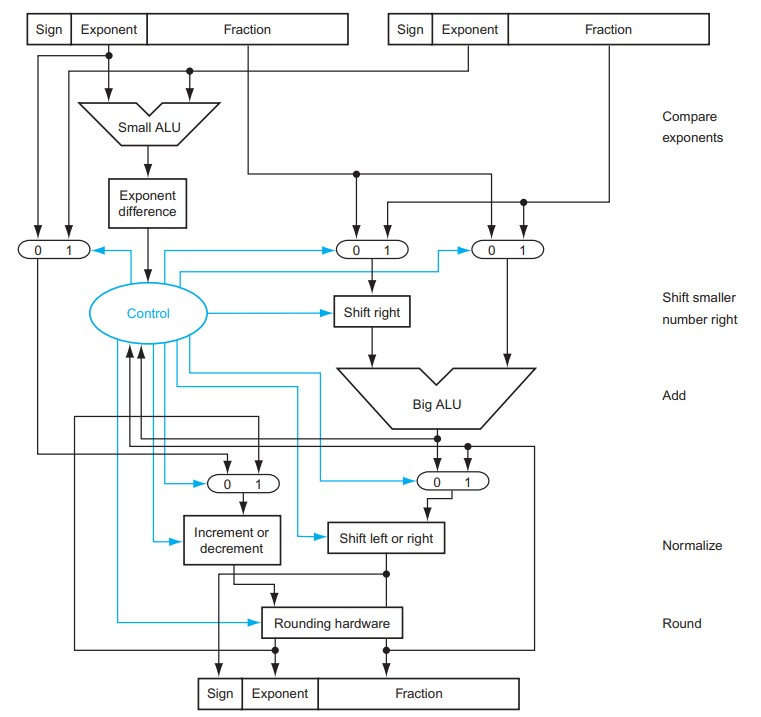
\includegraphics[width = 1 \textwidth] {ALU.jpg}
    \caption{HIGH-LEVEL BLOCK DIAGRAM}
    \label{fig:block}
\end{figure}


\begin{figure}[H]
    \centering
    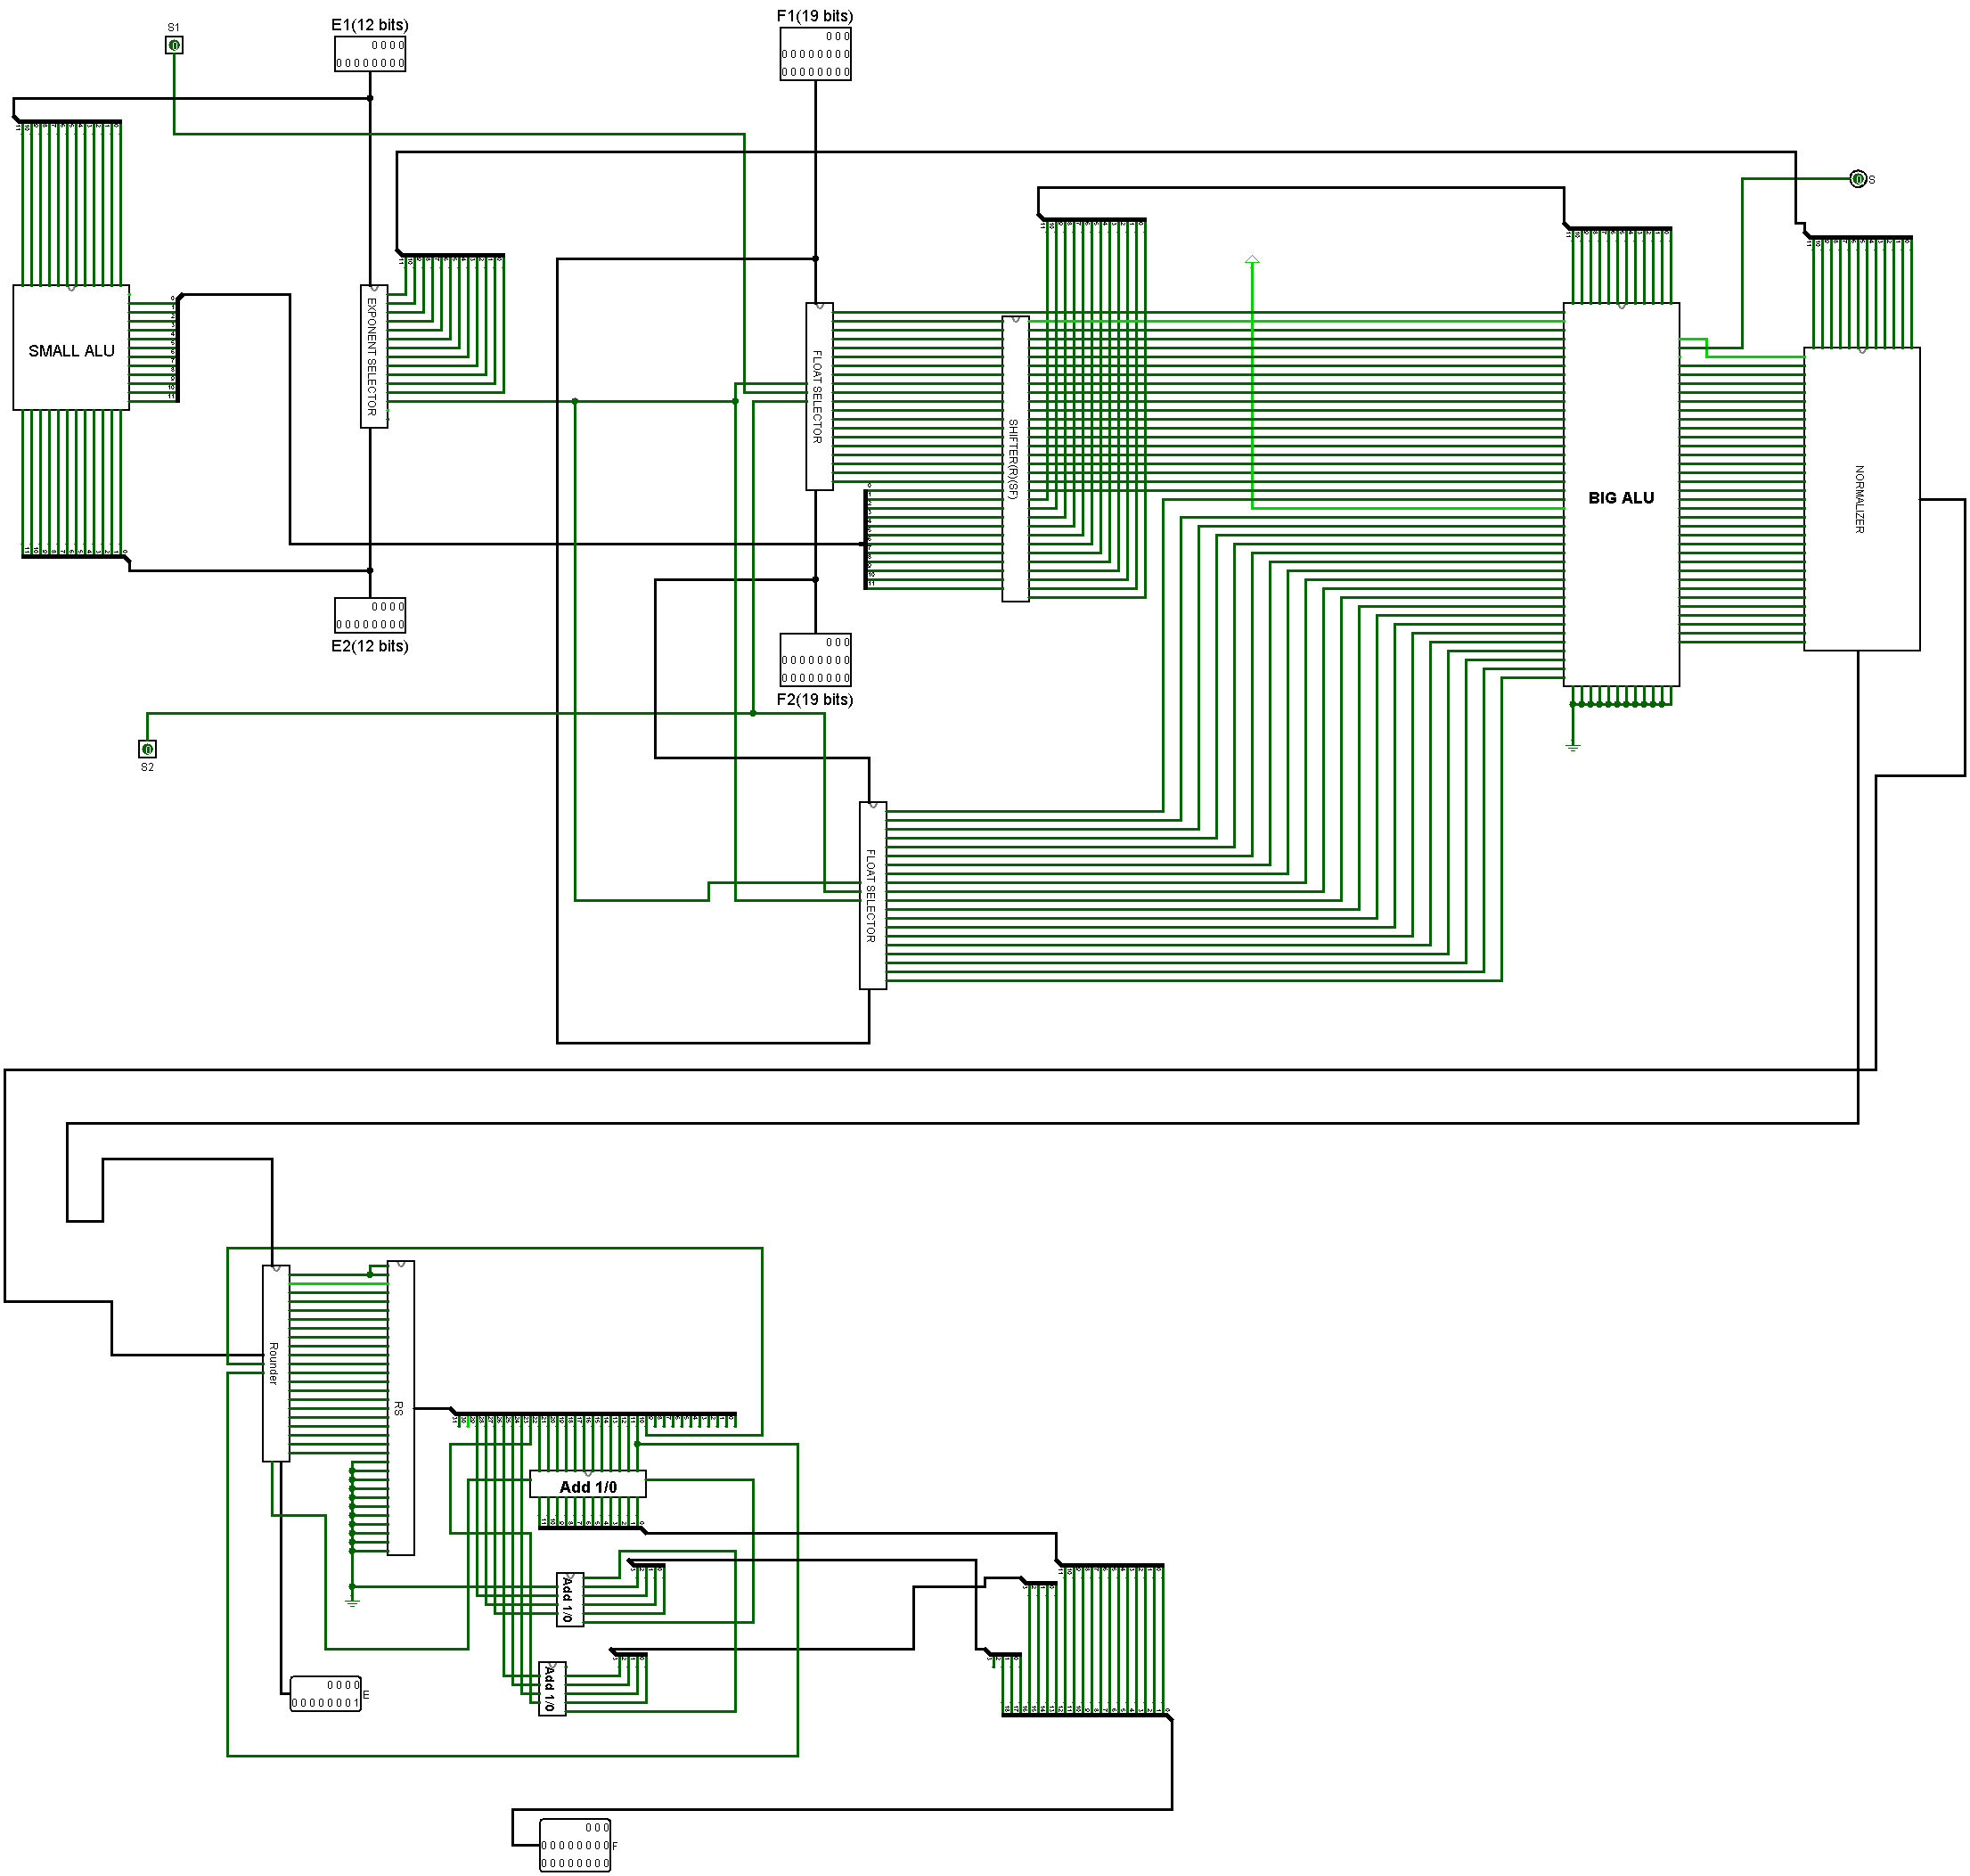
\includegraphics[width = 0.9 \textwidth] {BIG_BLOCK(100).png}
    \caption{BLOCK DIAGRAM FROM SIMULATOR}
    \label{fig:block}
\end{figure}

\section{Detailed circuit diagram of the important blocks}

\subsection{12 bit Comparator}

\begin{figure}[H]
    \centering
    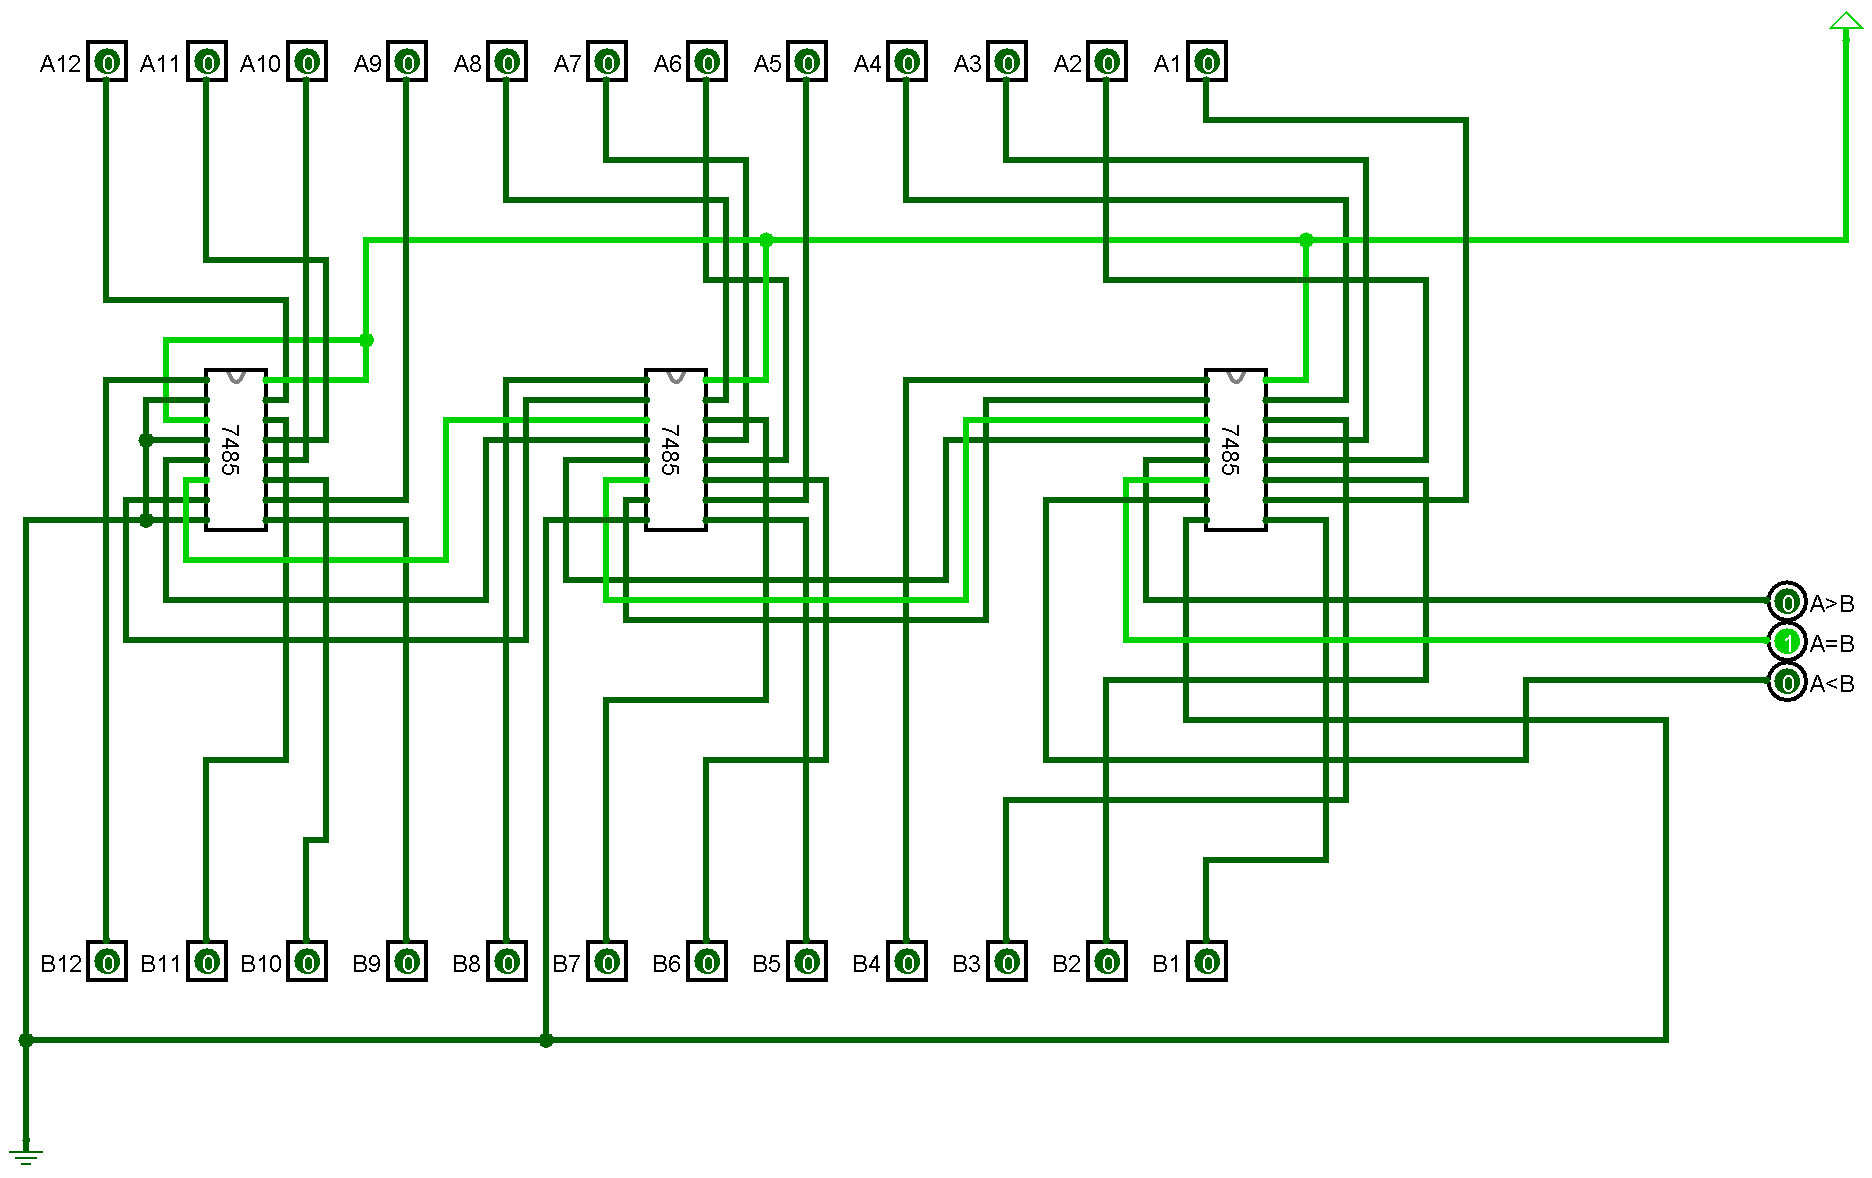
\includegraphics[width = 0.9 \textwidth] {Comparator.png}
    \caption{THE 12 BIT COMPARATOR}
    \label{fig:cmp}
\end{figure}

\subsection{Exponent Selector}

\begin{figure}[H]
    \centering
    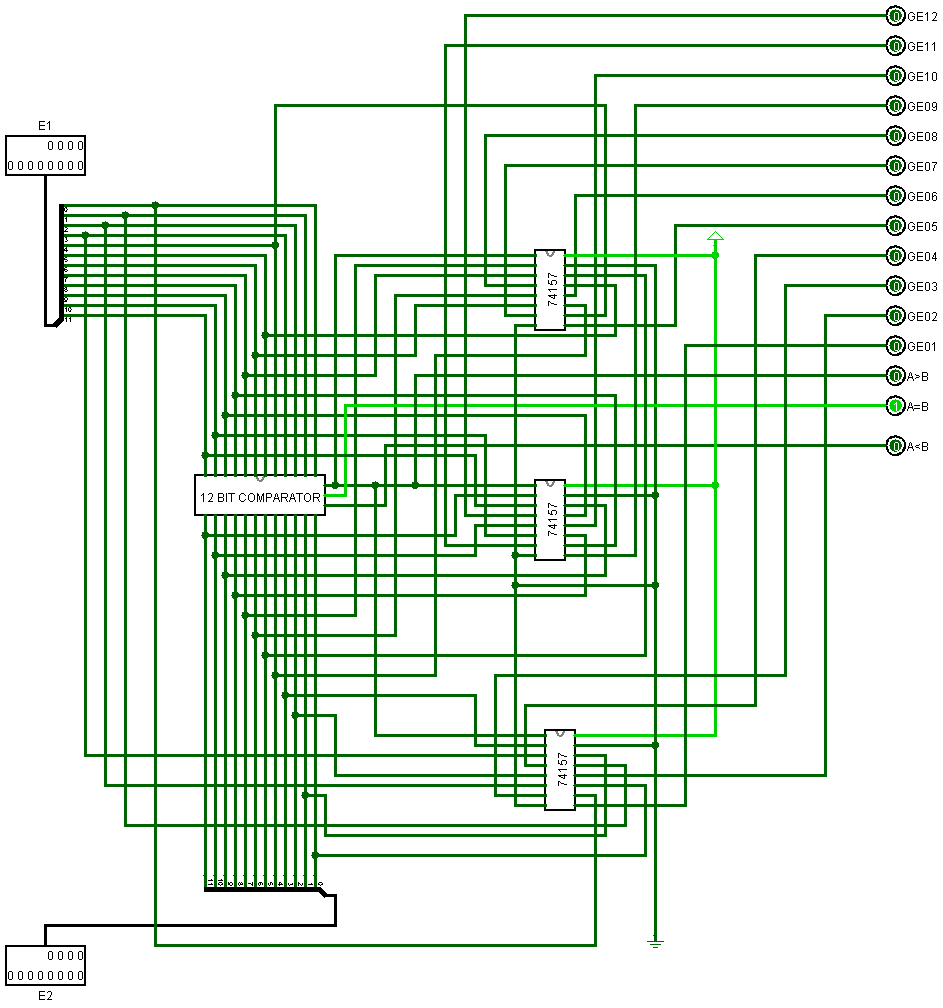
\includegraphics[width = 0.9 \textwidth] {ExpSel.png}
    \caption{EXPONENT SELECTOR}
    \label{fig:expctrl}
\end{figure}

\subsection{Float Selector}

\begin{figure}[H]
    \centering
    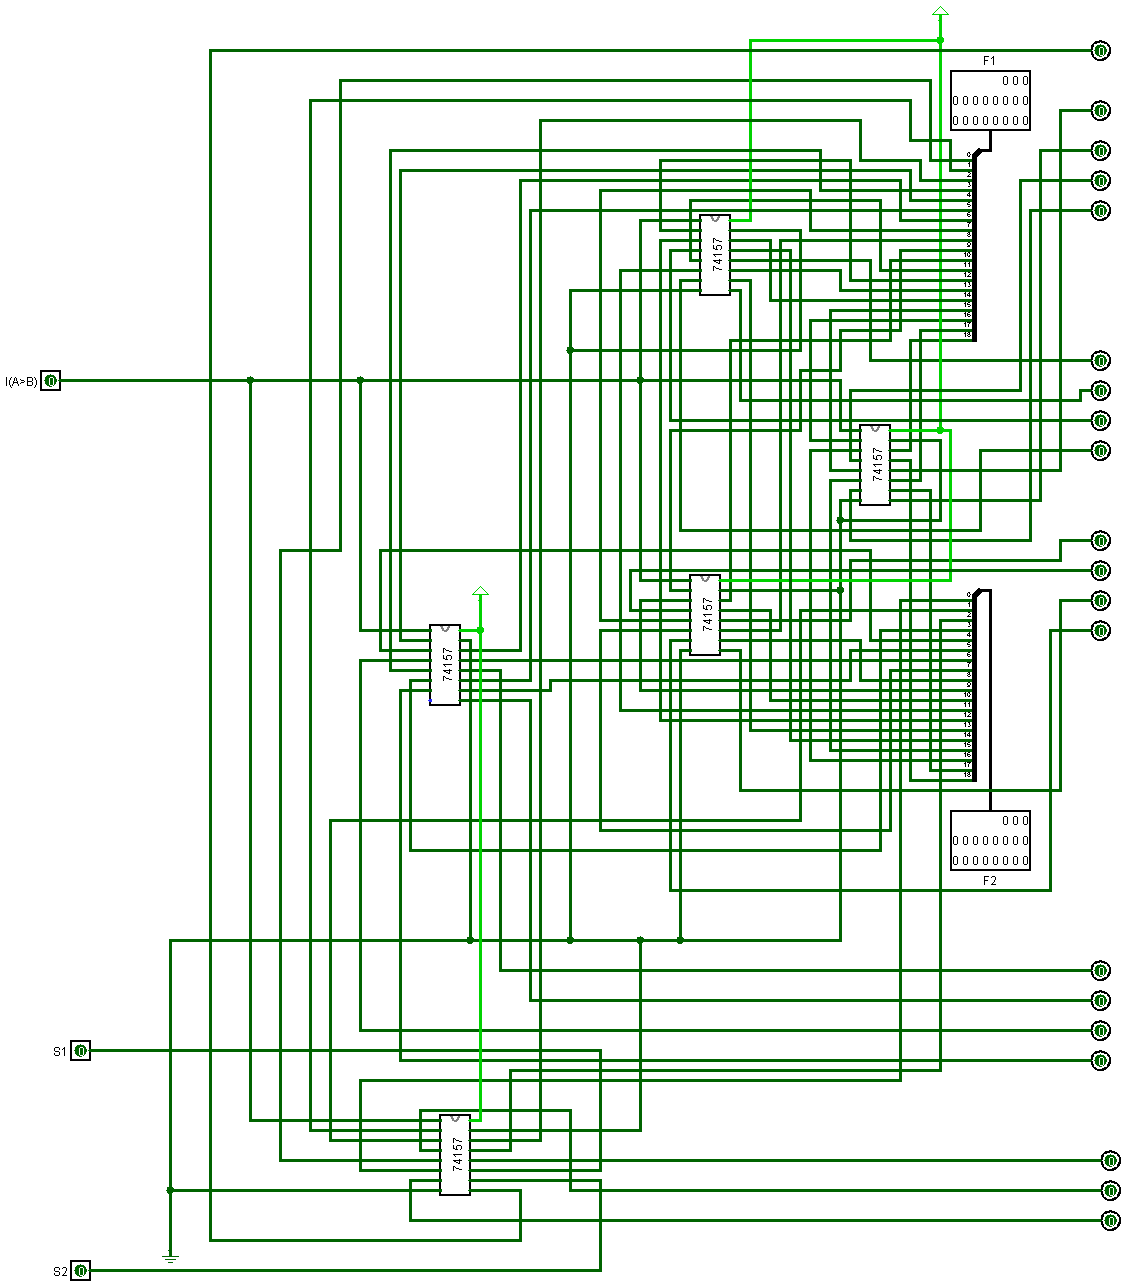
\includegraphics[width = 0.9 \textwidth] {Float selector.png}
    \caption{FLOAT AND SIGN SELECTOR}
    \label{fig:fsctrl}
\end{figure}

\subsection{Normalizer}

\begin{figure}[H]
    \centering
    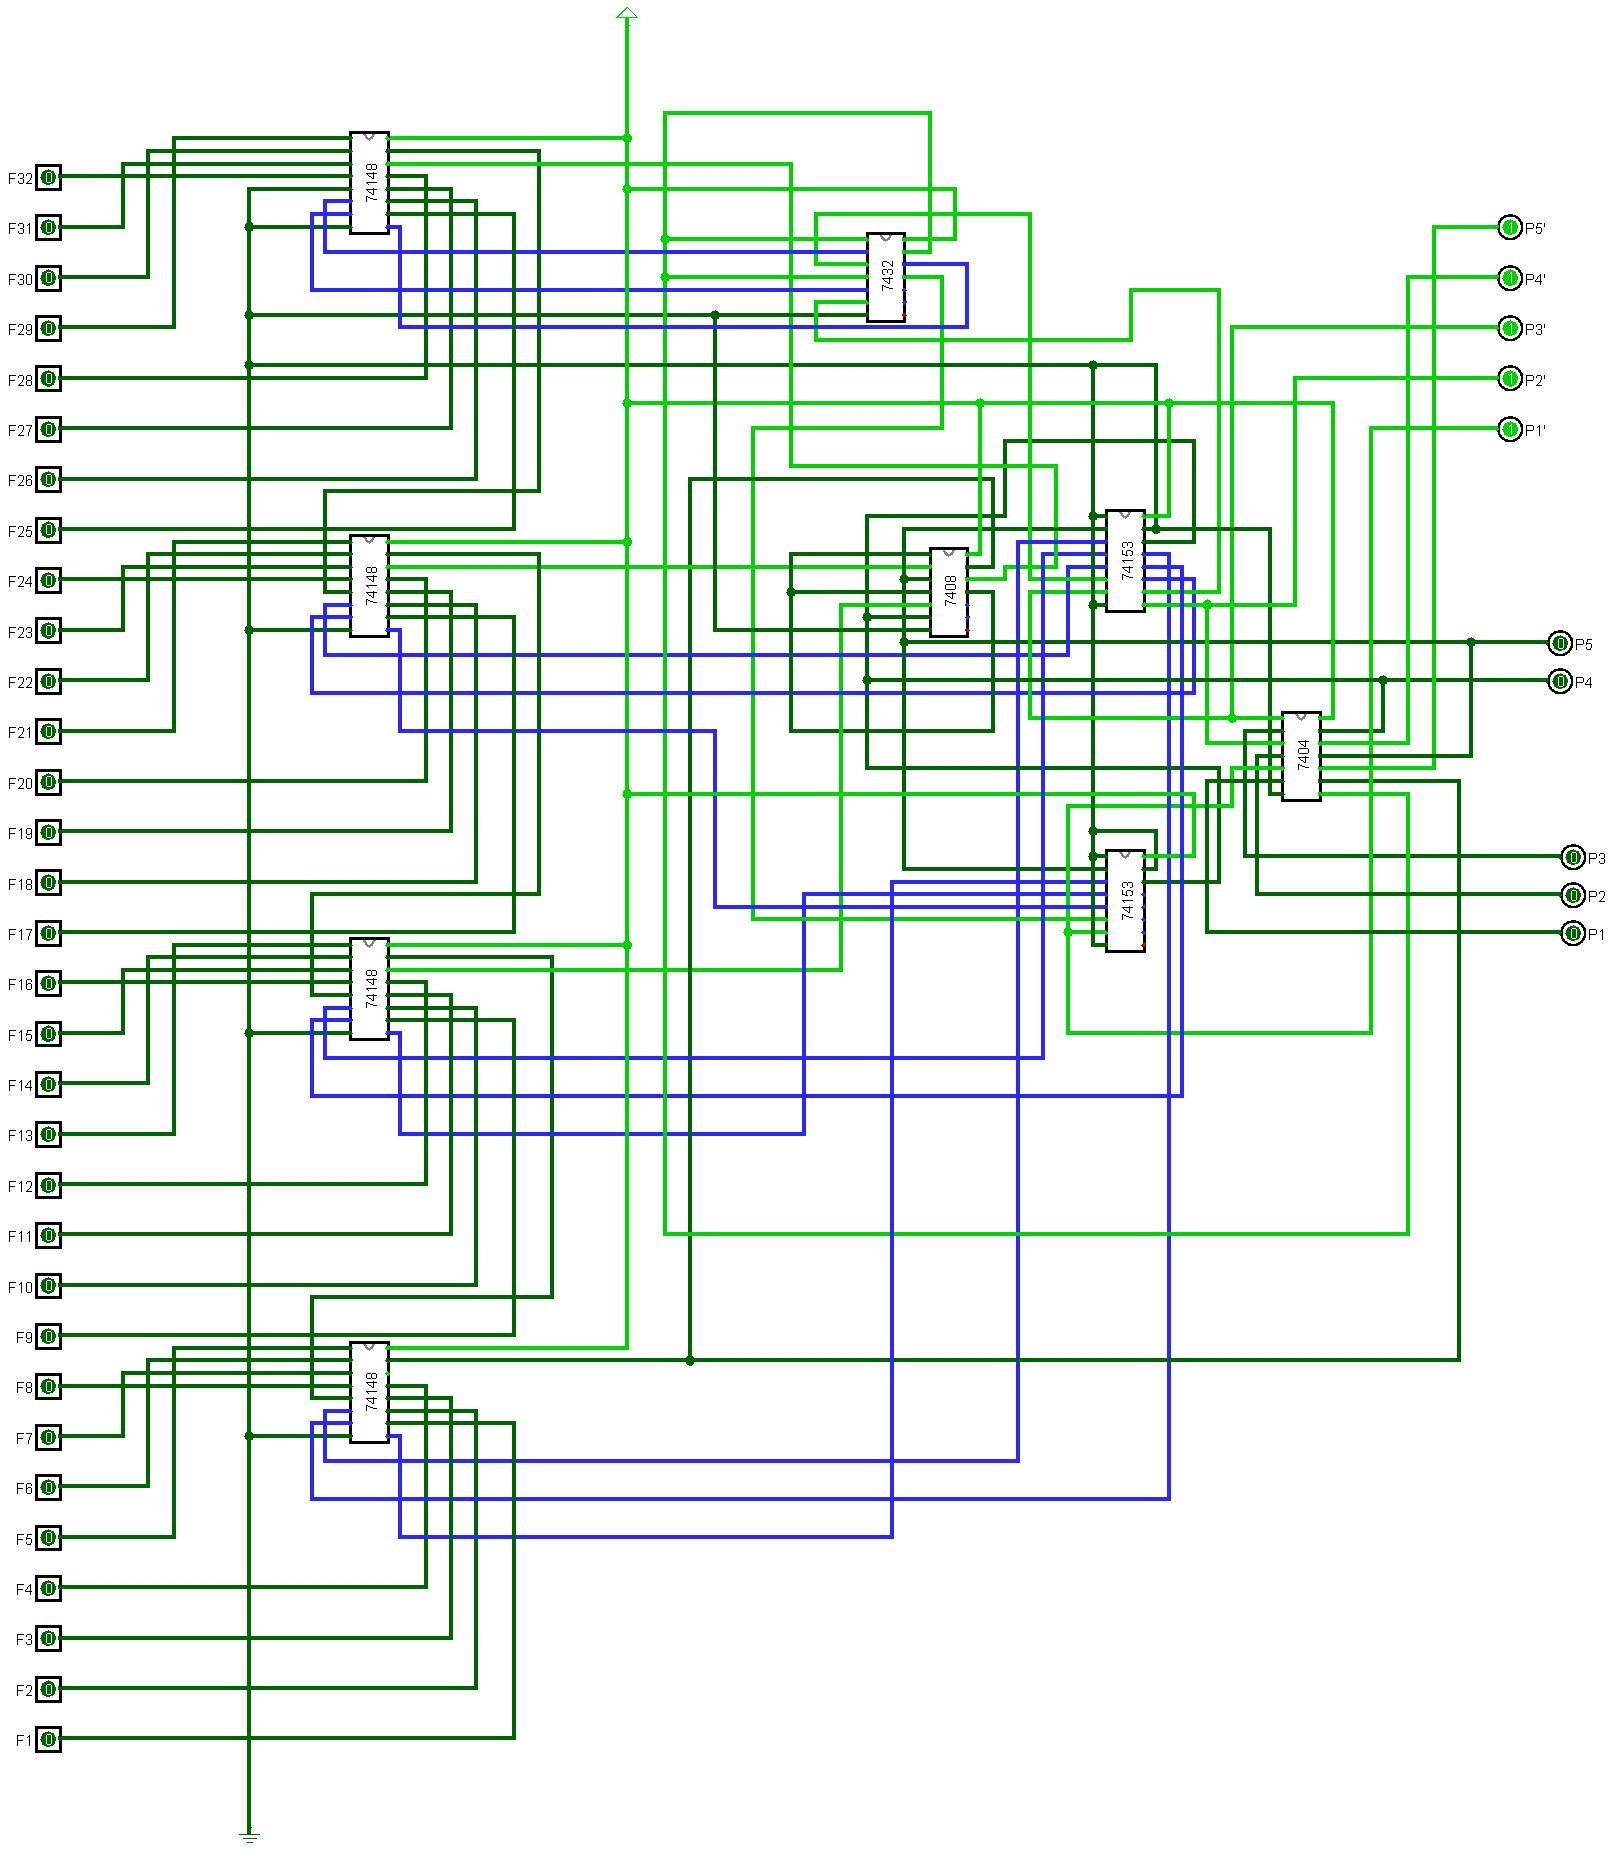
\includegraphics[width = 0.9 \textwidth] {PE.png}
    \caption{32*5 BIT PRIORITY ENCODER}
    \label{fig:pe}
\end{figure}

\begin{figure}[H]
    \centering
    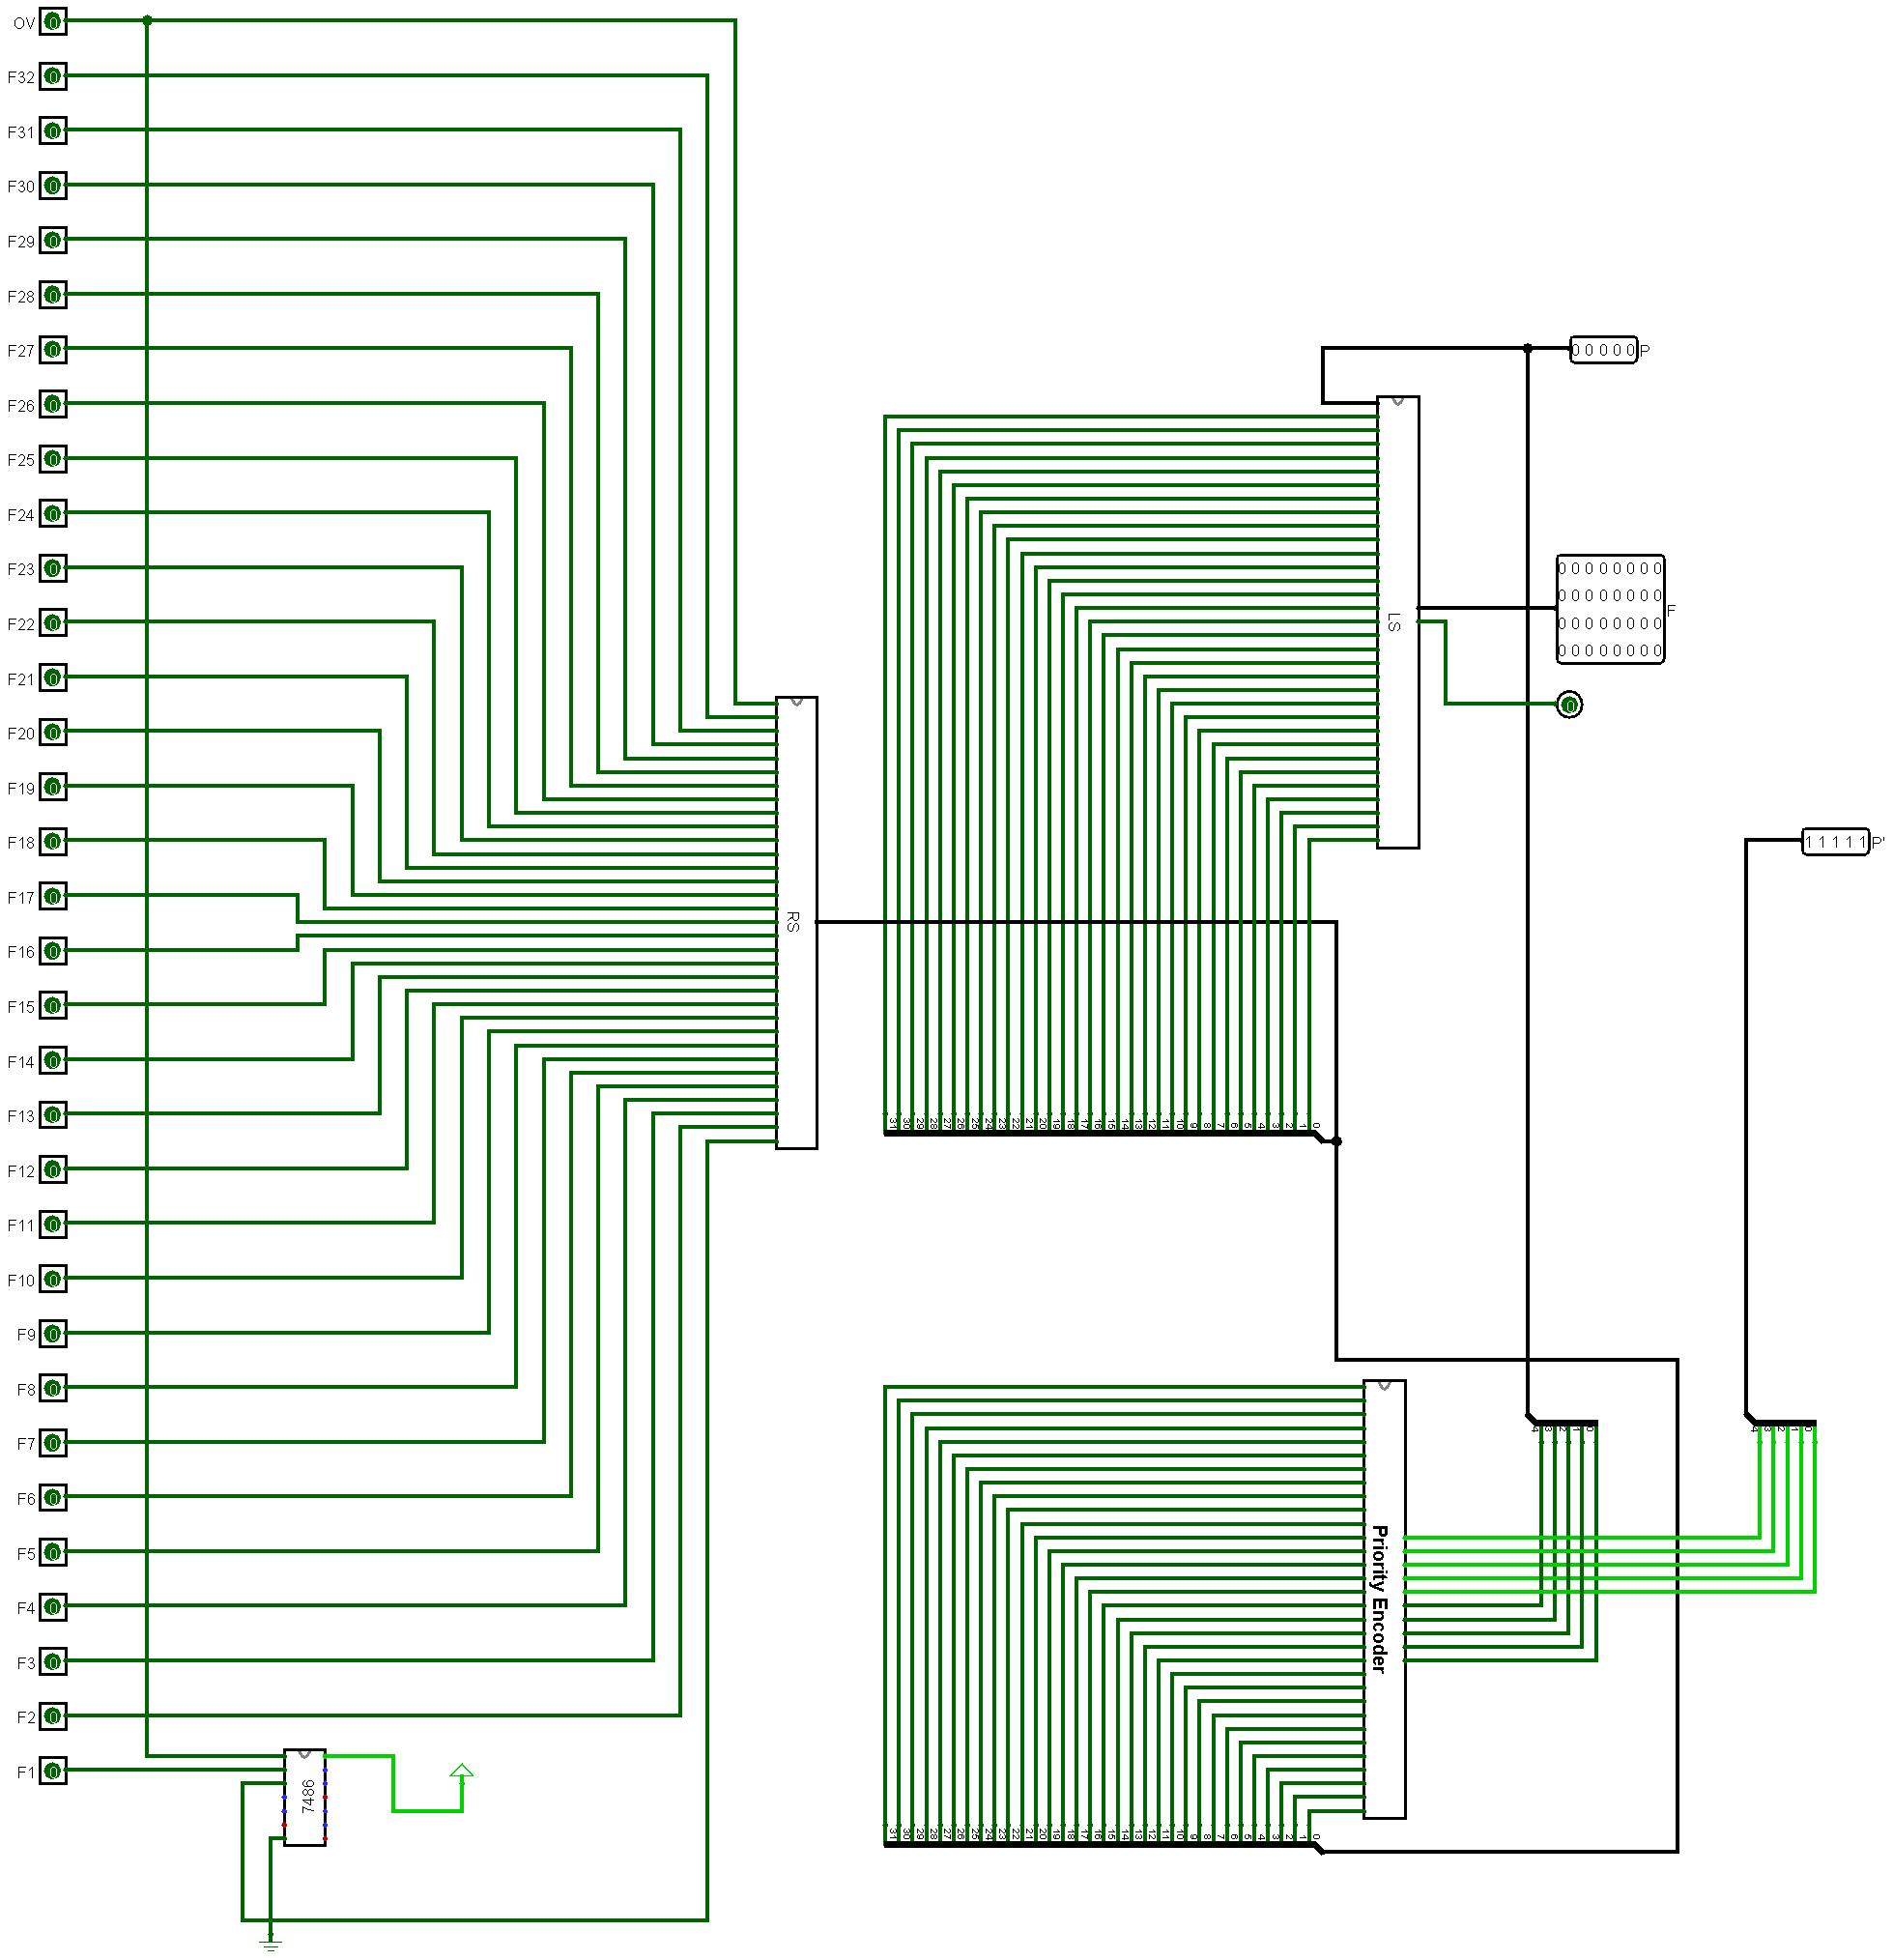
\includegraphics[width = 0.9 \textwidth] {NP.png}
    \caption{NORMALIZATION PRESTEP}
    \label{fig:np}
\end{figure}

\begin{figure}[H]
    \centering
    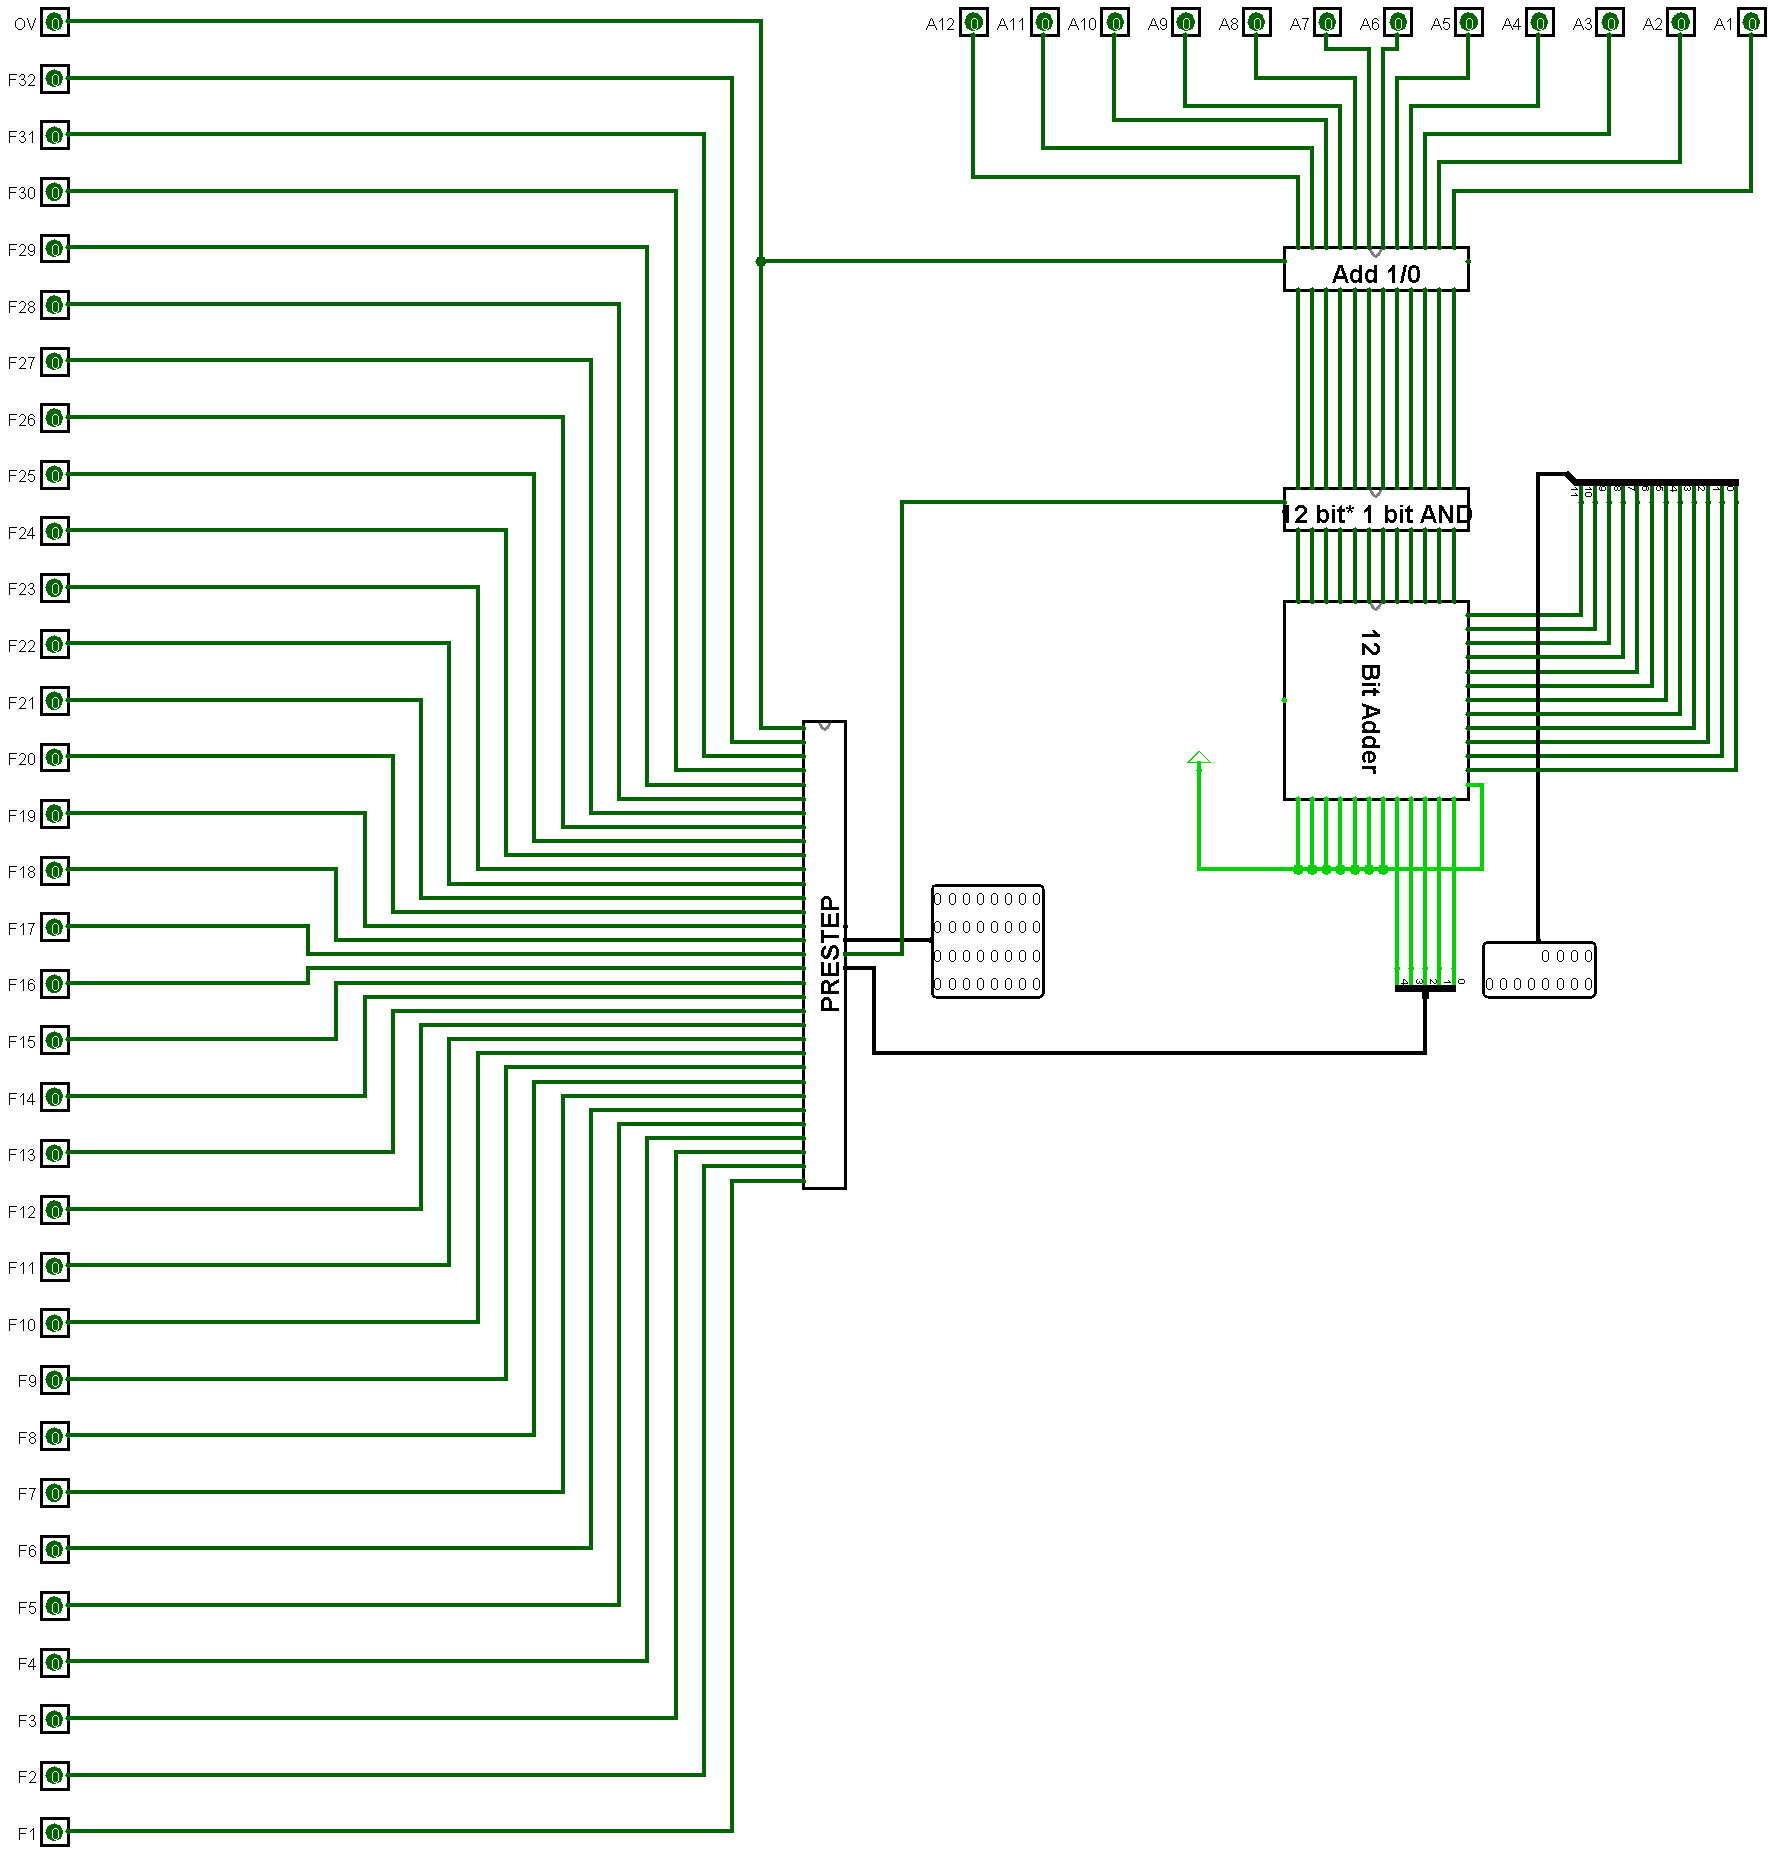
\includegraphics[width = 0.9 \textwidth] {NA.png}
    \caption{NORMALIZATION}
    \label{fig:na}
\end{figure}

\subsection{Rounder}
\begin{figure}[H]
    \centering
    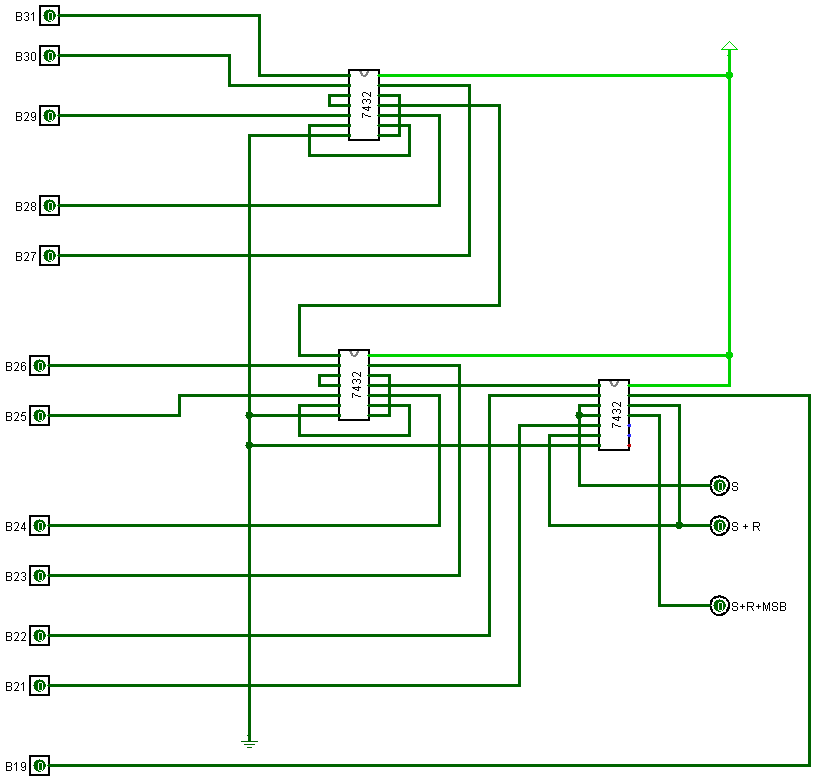
\includegraphics[width = 0.9 \textwidth] {Sticky OR.png}
    \caption{STICKY OR}
    \label{fig:so}
\end{figure}

\begin{figure}[H]
    \centering
    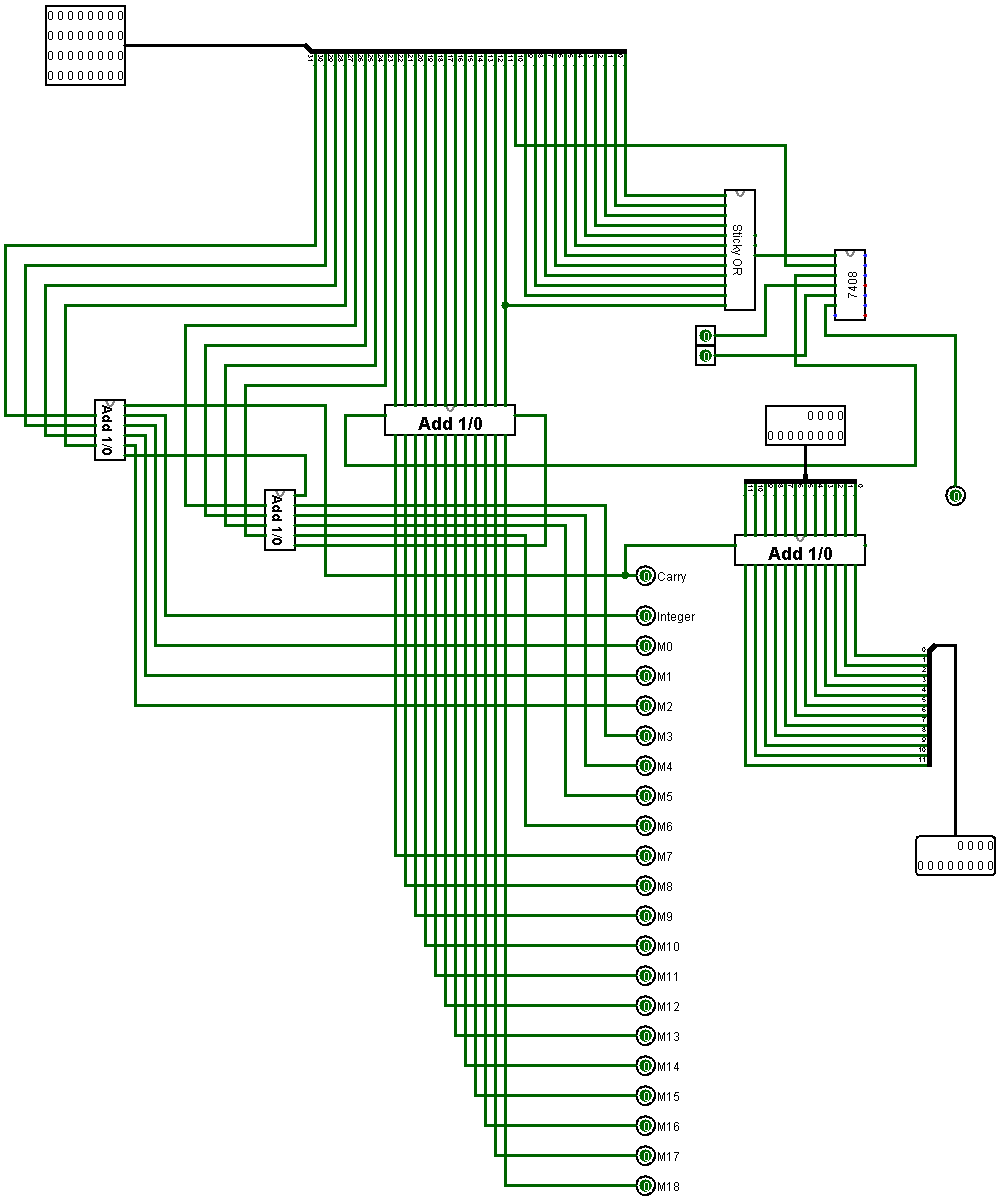
\includegraphics[width = 0.9 \textwidth] {Rounder.png}
    \caption{ROUNDER}
    \label{fig:rnd}
\end{figure}

\section{ICs used with count as a chart}


\renewcommand{\arraystretch}{2}
\large{
\begin{table}[H]

    \centering
    \begin{adjustbox}{width = \textwidth}
    
    \begin{tabular}{|c|c|c|c|}
    \hline
    
    BLOCK & SUB-BLOCK & IC & QUANTITY\\
    
    \hline
    \multirow{3}{*}{\makecell{Control }} & 12 bit Compressor & 7485 & 3 \\

    \cline{2-4}

    & \makecell{Exponent Selector\\(12 bit)}  & 74157 & 3 \\

    \cline{2-4}

     & \makecell{Sign and Float Selector\\(2*(19+1)bit)  
      (Both bigger and smaller)} & 74157 & 3*2=6 \\

    \hline
   \makecell{Small Number\\Right Shift}&\makecell{Priority Encoder\\(8*3)}&74153&1

   \\ \hline
    \multirow{6}{*}{\makecell{Normalizer \\ Pre-step }} & \multirow{5}{*}{\makecell{Priority Encoder \\ (32*5) }}  & 7404 & 1 \\

    \cline{3-4}

    &  & 7408 & 1 \\

    \cline{3-4}

    &  & 7432 & 1  \\

    \cline{3-4}

    &  & 74148 & 4  \\
    
    \cline{3-4}

    &  & 74153 & 2  \\

    \cline{2-4}

    & Others & 7486 & 1  \\

    \hline
     \multirow{3}{*}{\makecell{Normalizer\\Post-step}} & 12 bit Adder & 7483  & 3 \\

    \cline{2-4}

    & \makecell{Add 1 bit to 12 bit}  & 7483 & 3 \\

    \cline{2-4}

     & 12 bit * 1 bit AND & 7408 & 3 \\

    \hline
    
     \multirow{3}{*}{\makecell{Rounder}} & \makecell{Sticky OR\\(Finds S+R+L)} & 7432  & 3 \\

    \cline{2-4}

    & \makecell{Add (G(S+R+L))}  & 7408 & 1 \\

    \cline{2-4}

     & Add 1 bit to 20 bit & 7483 & 5 \\

    \hline

    {\makecell{Post Rounder\\ Operation}} & Add 1 bit to 20 bit & 7483  & 5 \\

    \hline

    \multicolumn{3}{|c|}{GRAND TOTAL IC COUNT} &
    49\\

    \hline
   
    \end{tabular}
    
    \end{adjustbox}
    \caption{Table For IC Count}
    \label{tab:ICtable}
\end{table} 
}
\renewcommand{\arraystretch}{1}


\section{Shifters and ALU used for the project}

\begin{itemize}
    \item \textbf{A 32 bit Logical Right Shifter : }\\

    This shifter is used in \underline{Small Number Right Shift} block, in order to match the exponents of addends and augends.

    \item \textbf{A 32 bit Roll Right Shifter : }\\

    This shifter is used in \underline{Normalizer Prestep} block, in order to roll right while there exists some overflow or carry. The xor of last bit and carry is taken to the foremost position after shifting only if there is a carry. That is if carry is 0 , then it results in no shifting as the binary number is already normalized. But if the carry is 1, then the output is normalized by 1 bit right shifting, and the complement of last bit rolls back.

    \item \textbf{A 32 bit Logical Left Shifter : }\\

    This shifter is used in \underline{Normalizer Prestep} block, in order to rotate left for normalization.

    \item \textbf{A 12 bit Exponent Difference determiner ALU : }\\

    This is the \underline{SMALL ALU} used in the assignment. It takes two 12 bit exponents as input and gives positive 12 bit difference as output.

    \item \textbf{A 32 bit Adder ALU : }\\

     This is the \underline{BIG ALU} used in the assignment. It takes two 32 bit matissa and their signs as input and gives positive 32 bit addition,carry flag, overflow and sign as output.
\end{itemize}


\section{simulator used along with the version number}

\subsection{Simulator Name}

\textbf{Logisim}

\subsection{Simulator Version}

\textbf{Logisim-win-2.7.1}

\subsection{Additional Libraries or Circuits}

\begin{enumerate}
    \item \textbf{7400-lib.circ : } This circuit file is a source of logisim IC's used for this Assignment.

    \item \textbf{SMALL ALU.circ : } This circuit file is the \underline{24*12} ALU , that takes two 12 but exponents as input and gives 12 bit greater exponent as output. The 12 bit Comparator used in this ALU is also separately used for the assignment to feed a control input based on which of the provided inputs is actually greater.


    \begin{outline}

         \1 \textbf{Inputs:}
    
        \2 12 bit input E1

        \2 12 bit input E2\\

        

        \1 \textbf{Outputs:}
        \2 12 bit output \textit{E1 - E2 : E2 - E1 ? E1 $>$ E2}\\
    
    \end{outline}

    
    

   \item \textbf{SMALL NUMBER RIGHT SHIFT.circ : } This circuit file is the \underline{31*32} circuit , that takes a 12 bit exponent and 19 bit mantissa as input and gives 32 bit floating point number as output, that results as an aftermath of 32 bit logical right shifting while equating exponent for the number with smaller exponent.

    
    \begin{outline}

        \1 \textbf{Inputs:}
    
        \2 12 bit input exponent

        \2 19 bit input mantissa\\

        

        \1 \textbf{Outputs:}
        \2 32 bit output floating point integer\\
    
    \end{outline}
    

     \item \textbf{BIG ALU.circ : } This circuit file is the \underline{66*35} ALU , that takes two 32 bit numbers and their signs as input and gives 32 bit sum and each one bit flag as output.

     
    \begin{outline}

    \1 \textbf{Inputs:}
    \2 1 sign bit for some input A
    \2 32 bit input A
    \2 1 sign bit for some input B
    \2 32 bit input B \\



    \1 \textbf{Outputs:}
    \2 32 bit output for A+B taking sign in consideration
    \2 \textit{Flags} 
    \3 1 sign bit for the output A+B
    \3 1 carry bit for the output A+B
    \3 1 overflow bit for the output A+B\\
  
    \end{outline}

     
\end{enumerate} 

These circuit files have been attached to the simulation submitted.

\section{Discussion}
All the ICs have been given proper power supply and ground. Subcircuits have been made to verify each step and to keep the block diagram as clear as possible. Important subcircuits have label on them so they can be identified easily. The floating point adder has been checked using several sample inputs and the output we got were correct. Thus, our floating point adder circuit has been built successfully.
\end{document}
